\chapter{Methodology}
\label{methodology}

This work looks at a case study which presents an issue directly related to the confidentiality of information when it is being stored in the cloud. It discusses the situation where it is important to be able securely store a secret value, as well as make modifications on it. A solution to the problem is proposed by employing homomorphic encryption. Then, it describes in a general way a proof of concept as a stand-alone solution. Afterwards, the scenario of using a client-server architecture is considered, discussing some decisions that were made regarding the communication needs. Relevant points on key management are mentioned, and also, how the tasks previously mentioned are being split by each component. 

The methodology in this work describes all the considerations and steps taken to build a solution to the problem analyzed from the case study. As such, the methodology has a very close relationship with the case study. Even though the object of study is the application of homomorphic encryption in the cloud, it is not trivial to find a fitting situation where it can be applied. The search becomes more complex as the limitations of state-of-the-art homomorphic encryption tools are considered. The case study that was thought of is simple enough so that the currently available tools can be used effectively, and complex enough so that applying homomorphic encryption is compelling and better than other alternatives.

\textbf{Case study}

The case study is explained as follows: a household commonly has more than one member, e.g. partner and children. The responsible members of the household (i.e. the parents) might want to keep an eye on the house while being away, especially if children are left behind. They would like to ensure that their children stay inside during this time, and that nobody else, except for a babysitter, enters the house. And if it were the case that somebody got in or out, they would probably wish to be promptly notified of it. This is especially true for the case when they are away for long periods of time, during a vacation, for example. A traditional solution consists in setting up a surveillance system throughout the house, which would certainly work to prevent robbery, but wouldn't necessarily work as a measure to know whether or not the children have left the house. Setting a surveillance system might be too costly for some families, and not be quite adaptive to their needs. It might be more efficient to deploy a system that detects when people enter and exit the building through the main door, and keep a counter of it. The main idea is that the \textit{surveillance count} gets initialized at some point in time, and, as people go in and out, the counter increases or decreases, respectively. Setting up the sensors and other pieces of hardware can be considered as a Do-It-Yourself project, as resources could easily be found. The issue comes out when the recorded data, that is, the counter, is to be accessed remotely via some kind of web application. 

[INSERT SAMPLE FIGURE]
% pendiente poner imagen

\textbf{Proposed solution}

The proposed solution addresses the issue hinted at the end of the study case description. This refers to making available the counter data to the householder without compromising confidentiality. Assuming that there might be more than one person who would have access to this data per household, it might not be appropriate to set up a Peer to Peer communication scheme. It makes more sense to have a server in the cloud that stores the counter data, waiting for requests from the clients to deliver the information. The data stored in the server is to be accessed from anywhere else; however, one of the most important aspects of the whole scheme remains unaddressed: confidentiality.

Usually, the householder would not allow others to know about the actual counter, including the server, as this information is considered to be sensitive. The traditional approach is to make use of public-key cryptography to encrypt the data and prevent from anybody else to know the counter. The counter value would then have to be encrypted using a certain cipher before it is uploaded to the cloud. However, this would imply that every time that there is a change in the counter, the whole ciphertext would have to be reuploaded to the server. Considering that person comes in and out of a building quite frequently, it would turn out to be a heavy burden which has an overhead cost that keeps accumulating every time there is an update. 

An alternative approach is to simply notify the cloud service of any changes that occur, so that it performs the addition or subtraction itself instead of relying on receiving the whole encrypted result. Even though this would not be possible to do with traditional cryptography, it can be done using homomorphic cryptography. The concept behind this approach is that, while initial counter value is being stored on the server, the client part that resides on the household sends over any change of individuals that are inside the building, and so the cloud service, i.e. the server, performs the appropriate homomorphic computations on the currently stored value. This occurs without the need of anybody reuploading the counter data again, and the server has no need of decrypting the data in the first place. Since the full ciphertext is not being resent, the overhead cost is reduced significantly.

Whenever the householder needs to know the value of the counter, he can authenticate with the cloud service to download the current ciphertext that represents the counter. The ciphertext can decrypted using the private key generated in the beginning. This aspect remains the same whether homomorphic encryption is used or not, and there is no way around it without compromising confidentiality. Considering that a system that detects when people come in and out might not be perfect, and if somehow the counter gets to an incorrect value, it could be reset to the correct amount. In this case, it would be unavoidable to send a newly encrypted counter value.

The solution itself consists in an implementation of a client-server software that aims to store and modify a secure counter by making use of homomorphic encryption. The various tasks that help reach this goal are distributed by the client and server components of the software. The client focuses initialization of the homomorphic encryption scheme, generation of public and private keys, encryption of initial counter data, among other things. On the other hand, the server is dedicated to store and manage the public key of the user and his current counter value. Both parts of the software utilize a library called HELib, which makes it possible to run homomorphic evaluations. In other words, this library is used perform basic operations on it, such as addition, subtraction, and multiplication. Consequently, it is also used to generate the public and private keys, encrypt data, and decrypt it. Once the encrypted counter is stored in the server, a different kind of client can then ask to download and decrypt it. It makes sense to say that it will be a different kind of client, since most likely the interested person would not be at the place where the counter was initialized.

\textbf{Details of the HELib library}

An implementation of an homomorphic encryption scheme, the Brakerski-Gentry-Vaikuntanathan (BGV), is openly available as a C++ library, called HELib. Using this library, it is possible to encrypt integer values and perform operations on them while being encrypted. There are many parameters to be considered when using this implementation, and these usually define how the public and private keys are going to be like. For this particular application, most parameters were left in their default values, as they seemed to serve the purpose. 

Part of the description in the code repository of HELib, it is stated that the library is considered to be low-level, and given its difficulty and constant changes, not that appropriate to use to build big applications with it.  [quote] 'At its present state, this library is mostly meant for researchers working on HE and its uses. Also currently it is fairly low-level, and is best thought of as "assembly language for HE". That is, it provides low-level routines (set, add, multiply, shift, etc.), with as much access to optimizations as we can give.'

It is important to note that the library recently started to support multi-threading, which would considerably speed up the evaluation times of the homomorphic operations. Not too long ago it started to support bootstrapping as well, a technique that prevents the ciphertext from getting too much noise and results in the incorrect evaluation of the operations.

\textbf{Setting up the parameters and context}

The HElib library is an implementation of a homomorphic encryption scheme, and as such, it has certain requirements before it can encrypt data or even generate keys. First of all, it has a list of parameters which must be manually set. Depending on the parameters applied, some aspects that directly affect the keys and ciphertext are altered. The suggested values are used for the majority of the parameters. Altering the values of the parameters could be an interesting way to do experimentation with the key size and computation time required.

The following table briefly describes each parameter used in HElib. It does not go into much depth, as those details are mostly pertaining to the algorithms in the library.

%\begin{table}
  \begin{tabular}{|l|c|r|}
    \hline 
    R  &     number of rounds &  default=1     \\ \hline
    p  &     plaintext base  & default=2  \\ \hline
    r  &     lifting  & default=1  \\ \hline
    d  &     degree of the field extension  & default=1  \\ \hline
    c  &     number of columns in the key-switching matrices  & default=2  \\ \hline
    k  &     security parameter & default=80  \\ \hline
    L  &     number of levels in the modulus chain  & default=heuristic  \\ \hline
    s  &     minimum number of slots  & default=0  \\ \hline
    repeat &  number of times to repeat the test & default=1  \\ \hline
    m   &    use specified value as modulus & optional  \\ \hline
    mvec &   use product of the integers as  modulus & optional \\ \hline
    gens &   use specified vector of generators & optional \\ \hline
    ords  &  use specified vector of orders & optional \\ \hline
  \end{tabular}
%  \caption{Parameters used for use of HElib}
%\end{table}


\textbf{Key generation and serialization}

As this library requires the use of public and private keys, the user is required to create his own set of keys, and it is only the public key which he should be willing to share. The user then shares his public key with the cloud service by some means of registration, so he does not have to share it every time he makes use of the service. The public key is used to encrypt the counter data for the first time before sending it over to the server, and the server itself requires this public key in order to perform the homomorphic operations.
The generation of the keys is pseudorandom, so extra care should be taken as to not to use a predictable seed, so that the public and private keys are not recreated by someone else. 

After instantiating context with all the necessary parameters, the set of keys can be generated. Firstly, the public key is obtained by simply instantiating an object of the class \textit{FHESecKey}. Then, a copy of the public key is made as the foundation for the private key. This copy makes use of a method called \textit{GenSecKey(w)}, which takes \textit{w} as a seed to create the real private key. Finally, it goes through a process that computes key-switching matrices, which are used in the internal algorithms of the library.

\begin{lstlisting}
  publicKey = new FHESecKey(*context);
  secretKey = publicKey;

  secretKey->GenSecKey(w); 
  addSome1DMatrices(*secretKey); 
\end{lstlisting}

Before proceeding to encrypt the data, it is important to have the public key serialized and ready to send it to the server. Serialization is a popular term used to describe the encoding of objects and the objects reachable from them, into a string of bytes. It is commonly used for lightweight persistence and for communication via sockets 
[reference: http://docs.oracle.com/javase/8/docs/technotes/guides/serialization/index.html ]. In this case, it is used as a means of temporarily saving the public key in a stream of bytes so it can be shared with a remote server that will be able to read such stream. Only after the contents of the saved object have been fully read, it is possible to reconstruct the public key. Fortunately, the HElib provides a very simple way to do serialization, since the class 
\textit{FHESecKey} supports the \textless\textless operator which works quite nicely with a couple popular serialization class in C++ called \textit{istringstream} and \textit{ostringstream}. The use of this class is showed as follows: 


\begin{lstlisting}
  ostringstream pkstream;
  pkstream << *publicKey;
\end{lstlisting}


This way, the data of the attributes found in the public key object has been stored as a stream of bytes in a highly portable object from the \textit{ostringstream} class. Using this newly populated object, the public key can be shared using sockets.

\textbf{Encryption of the Counter Value}

In order the protect the value of the counter from being known from other parties, including the server itself, it must be encrypted. This means that an encryption algorithm, provided by the HElib, is to be used on the plaintext that represents the counter. The result of this process is a ciphertext, which, unless provided with the corresponding private key, cannot be brought back to its plaintext form. 

Following the conventions defined in the HElib, an object from the \textit{EncryptedArray} is initialized using the \textit{context} and \textit{G} which were previously set. \textit{EncryptedArray} can be seen as a container for the plaintext, where the value of the counter is placed. Once it has been done, a method called \textit{encode} of the same class can be used to prepare the data for encryption. The ciphertext is stored in a different kind of container, which comes from the class \textit{Ctxt}. This container is initialized using the public key as argument. Afterwards, the encryption of the plaintext data can be done using a method of the \textit{EncryptedArray} object simply called \textit{encrypt}. This method receives as arguments the objects of the plaintext and ciphertext containers, and the public key.

\begin{lstlisting}
  EncryptedArray ea(*context, G);
  PlaintextArray counter(ea);  
  counter.encode(people);
  Ctxt& encryptedCounter = *(new Ctxt(*publicKey));  
  ea.encrypt(encryptedCounter, *publicKey, counter); 
\end{lstlisting}

This ciphertext can be used in several ways: its value can be modified by adding, substracting or multiplying it by some arbitrary value, it could also be decrypted at any time using the private key, or it could be serialized as it was done with the public key, so another party, e.g. the server, can receive and store it.

\textbf{Single component operation flow}

Before attempting to break down the whole implementation in two parts: the server and client side, a proof of concept was implemented which combined the tasks of both parts into a single program. The flow of this program represents how the data gets transformed through several tasks. 

\begin{enumerate}
	\item Parameters to use with the HELib are arbitrarily chosen, while other required values are computed.
	\item Context of the HELib library is set.	
	\item Public and private keys are created using the context.
	\item Optionally, public key can be serialized into a file so it can be used later.
	\item The structures to store plaintext and ciphertext are declared.
	\item The initial counter value is set into the plaintext structure.
	\item The plaintext is encrypted using the public key and stored into the ciphertext structure.
	\item Values are arbitrarily added or substracted from the ciphertext.
	\item Ciphertext is decrypted using the private key, and its value is stored in another plaintext structure.
	\item Newly decrypted plaintext is printed to verify correct result from operations.
\end{enumerate}

\textbf{Software Architecture and Data transmission}

Even though the case study started out considering cloud services, an actual implementation of the application can be addressed with a client-server architecture. The client-server architecture is a popular model that consists of a two parts: a client and a server. Usually, the server just waits for any kind of request from a client to do some kind of task. Meanwhile, the client usually starts some kind of task, but depends on the server to do it completely. Most of the time, the client depends on the server because it might have something that the client does not, like a database.

In this case, the implementation of the counter application is approached using a client-server model. The server represents the cloud service that stores and modifies the encrypted data on request, while the client plays the part of obtaining and encrypting the sensitive data. The client also takes care of tasks such as initializing the homomorphic encryption context, generating the public and private keys, encrypting the data, and serializing the encrypted counter before sending it over to the server. Meanwhile, the server takes care of establishing the communication details via TCP sockets, reconstructing the received ciphertext, and performing operations on it. Although a more secure implementation would consider using the Secure Socket Layer (SSL) over TCP, it was simplified to cover only the details pertaining the use of homomorphic encryption.

Once the user has obtained the initial data, i.e. by counting the number of people currently in the house at a given time, he proceeds to feed the data to the client program, so it is encrypted using the previously generated public key. After the counter data has been encrypted successfully, the data is then sent to the server via sockets. There were two possible protocols that could have been used for this part: UDP and TCP. UDP stands for User Datagram Protocol and is used in conjunction with the Internet Protocol. UDP works best when the data units that are being sent are very small. It is also a little bit problematic considering that it does not reassembles data packets once they have arrived at the destination. The other option that was considered was TCP, which stands for Transmission Control Protocol. It is a little friendlier to use in the sense that it reassembles datagrams in the correct order once they arrive at their destination. However, it adds a little bit of overhead cost since it adds a header section per segment. In the end, it was chosen to use TCP over UDP, especially since it might become complicated to keep track of the order of the data packets.

\textbf{Sending and reading serialized data}

The serialized data that is sent through sockets was very large to be done with a single function call, which is why a few considerations have to be made on the implementation. It is recommended to have some kind of supporting function that continuously is attempting to send data to the server, until there are no bytes left.

The following snippet of code shows how the ciphertext is serialized using the \textit{ostringstream} class, and then a function call is made to a supporting function which continuously attemps to send all the remaining bytes to the server. It is relatively simple to keep track of how many bytes are being sent and how many are left, which is why it stops sending data at the appropriate time.

\begin{lstlisting}
  ostringstream oss;
  oss << encryptedCounter;

  if(sendalldata(sockfd, oss.str().c_str(), &msgsize) == -1) {
    printf("ERROR. Only \%d bytes sent!\textbackslash n", msgsize);
  }

int sendalldata(int s, char const* buffer,  int *len)
{
  int total = 0; // bytes sent
  int bytesleft = *len; // bytes left to send
  int n;
  
  while(total < *len) {
    n = send(s, buffer+total, bytesleft, 0);
    if (n == -1) { break; }
    total += n;
    bytesleft -= n;
  }
  *len = total; 
  if(n == -1) 
    return -1;
  else 
    return 0;
}
\end{lstlisting}

As it cannot be expected that the serialized ciphertext of great size will be succesfully sent with a single send function call, the same goes for the receiving end. Certain measures have to be taken so that all the data is received complete and in the appropriate order.

The following piece of code extracted from the server side of the software goes through the part where the ciphertext is being received after it has been serialized. First of all, a buffer is declared and initialized with the size of the ciphertext, which was previously received. A function called \textit{bzero()} is used to prepare and empty the buffer.  Then, a while loop is done as long as there are bytes remaining to be received. As more iterations go by, more data is appended to the buffer. A couple of variables are used to keep in check how many bytes have been read and how many are still pending to be read.

\begin{lstlisting}
  char* responseBuffer = new char[responseBufferSize];
  bzero(responseBuffer, responseBufferSize);
  bytes_read = 0;
  int bytes_remaining = responseBufferSize;
  int this_recv;
  while(bytes_remaining > 0) {    
    this_recv = recv(newsockfd, responseBuffer+bytes_read,
                bytes_remaining, 0); 
    if(this_recv <=0) error("error on receive");
    else {
      bytes_remaining -= this_recv;
      bytes_read += this_recv;
    }
  }
\end{lstlisting}

\textbf{Reconstructing the ciphertext}

It was mentioned before that serialization allowed persistence and made it easier for object data to be sent via sockets. However, the serialzied objects cannot be used the way they are received. In this case, the ciphertext was serialized before being sent to the server, and once it is properly received, the data must be used to reconstruct the original ciphertext object.
If this is not done, there is no way to perform operations on the ciphertext, or even decrypt it to know its value.

The following piece of code describes the steps to be taken in order to reconstruct the object that can contain the ciphertext. First of all, the buffer that was previously filled with data is then copied into a string variable, then it goes through a couple of steps so it can be used as a \textit{istringstream} object. The preparation is certainly more complicated, but the reconstruction of the object is quite simple itself. Since HElib is friendly with the \textgreater\textgreater operators, it can be done in one step. This operator basically takes the data from one variable and puts it in another kind of variable, one being a \textit{istringstream} object, and the other a \textit{Ctxt} object.

\begin{lstlisting}
  string strBuffer((const char*) responseBuffer, bytes_read);
  istringstream serialCipher;
  serialCipher.str(strBuffer);

  Ctxt receivedCipher(publicKey);
  serialCipher >> receivedCipher;
\end{lstlisting}


\textbf{Changes in the counter}

Once the initial value of the counter has been received by the server, there are two possible scenarios that could occur next: the value gets viewed by the householder, or a change in the counter occurs. Whenever a significant change is observed by the client program, the change is promptly notified to the server, which could be either positive or negative. When the cloud service receives the value of change, it either adds or subtracts it from the previously stored value. The change is immediately visible to the householder who might wish to know the current value of the counter.

As the implementation of the counter was started before December 2014, bootstrapping was not considered to use. Bootstrapping is an advanced technique in fully homomorphic encryption which allows more homomorphic evaluations to be run on a ciphertext. As it has been mentioned, whenever a homomorphic evaluation is performed on the ciphertext, a small amount of noise is added to it, and after a certain threshold, the ciphertext becomes unusable, in the sense that it no longer decrypts back to the correct value. As an alternative to bootstrapping, however, it is possible to reset the counter, i.e. upload a newly created ciphertext with an initial counter value, so that more homomorphic evaluations can be performed on it. Considering that the operations that will be done most of the time are addition and subtraction, this is not something that will occur often, but eventually will. 

\textbf{Architecture breakdown}

The proof of concept that makes use of homomorphic encryption ends up being completely linear in the sense that it has no communication at all with different parts of the outside world. The considered case study implies that there is both a household where the counter is initialized and another location where the current counter value can be accessed. Considering this aspect, it makes sense to have a server in the cloud that can be accessed securely which will contain the current value of the counter for each household. This requires the server to store the public key as well, since to be able to modify the ciphertext of the counter data, such a key is needed. 

In the following figure, a breakdown of the client-model architecture employed is depicted. As previously mentioned, the solution is split into two parts: client and server sides. Each side has specific tasks that must be performed independently. The figure was conceived as an attempt to organize the software structure and assign a functionality to one of the components. The client side is in charge of the tasks that are performed at the place where the counter is initialized, i.e. the household. Such tasks include: setting up the parameters and context required by the HElib, generating the set of public and private keys, registering the public key, encrypting the initial counter value, serializing the ciphertext, recording changes in the counter value, and decrypting the received ciphertext. 

\begin{figure}[h!]
  \centering 
  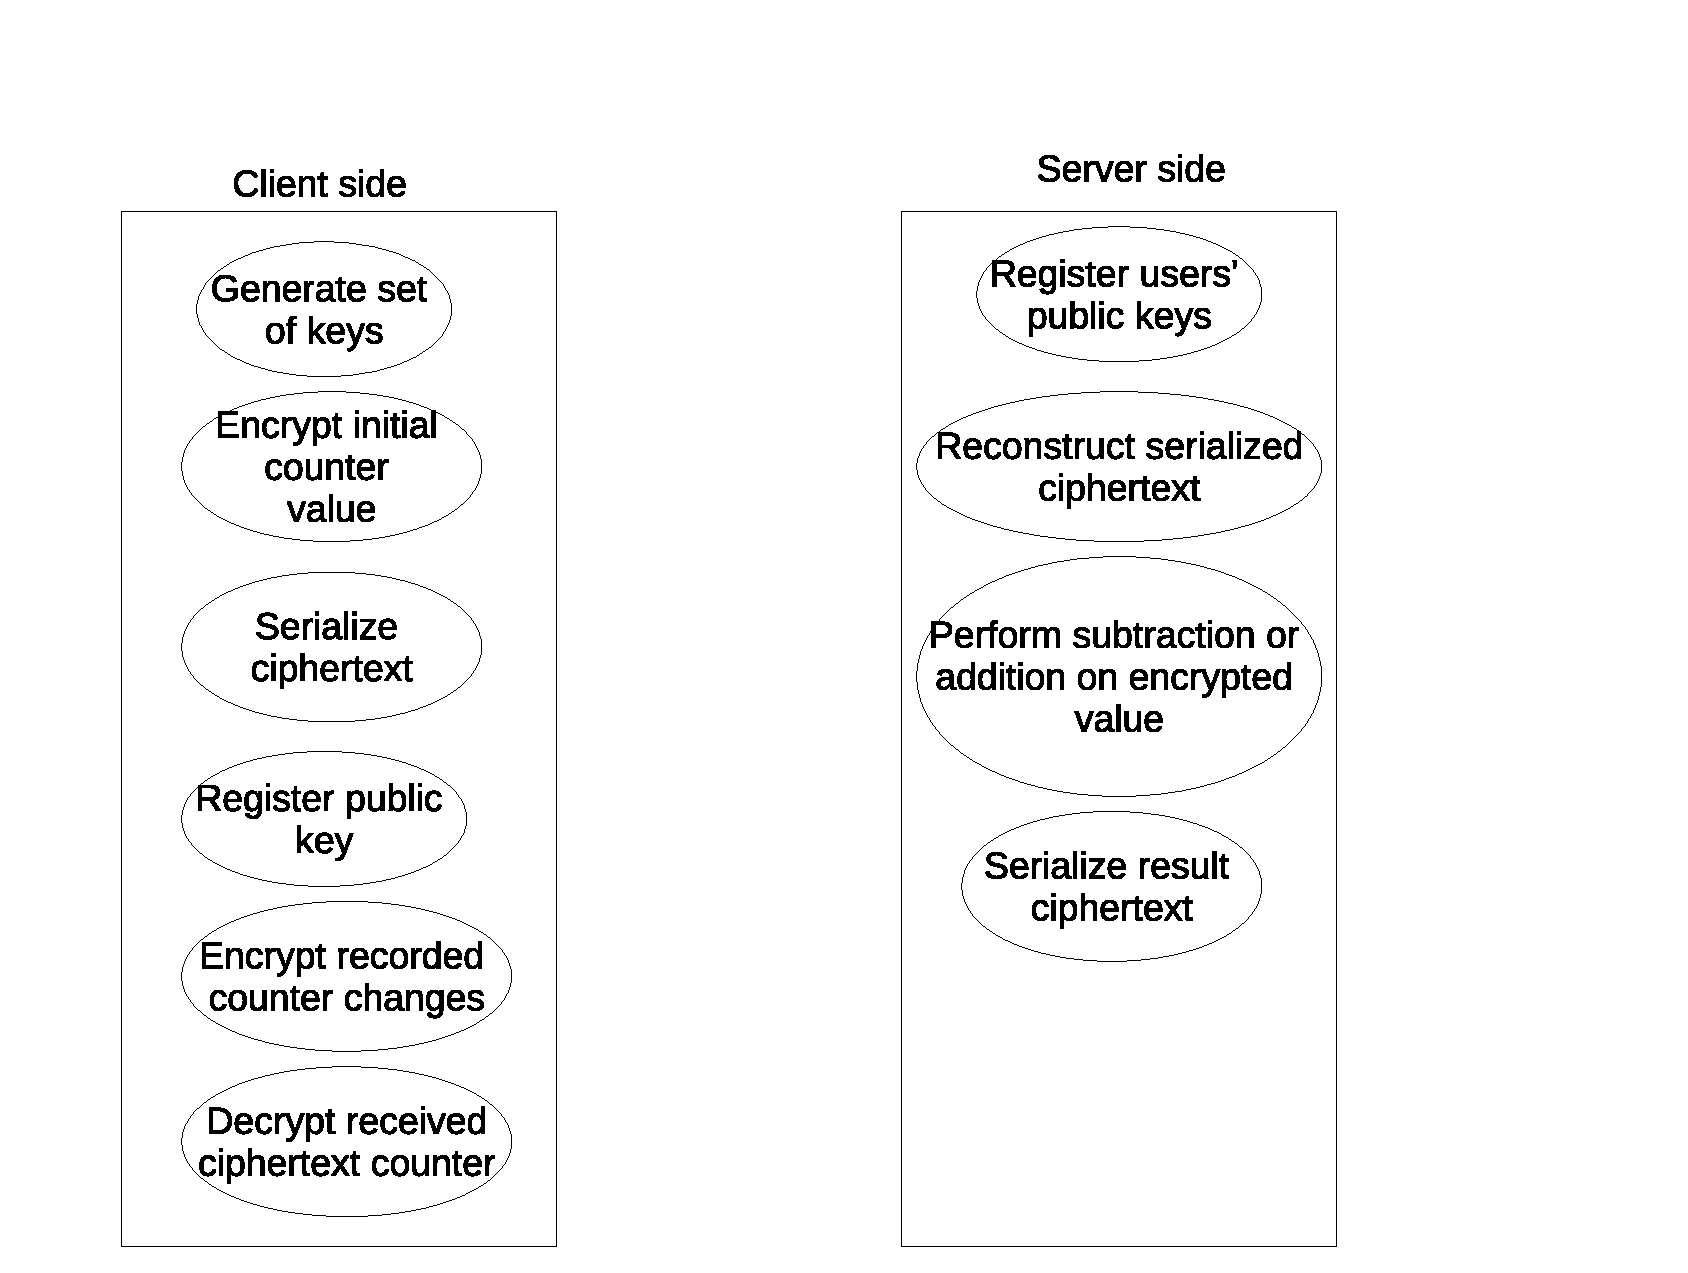
\includegraphics[scale=0.7]{clientserver}
  \caption{Architecture breakdown into client and server.}
\end{figure}

[ADD SEQUENCE DIAGRAM AND DESCRIPTION]

%\begin{figure}[h!]
%  \centering
%  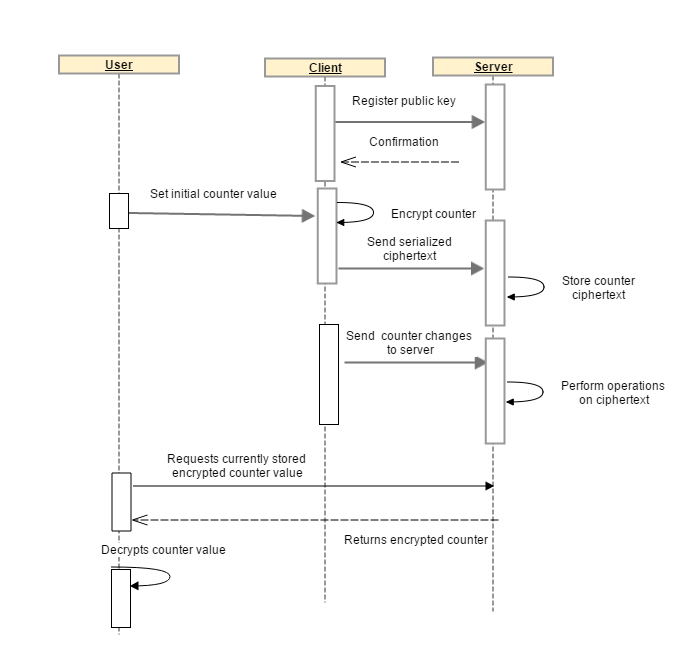
\includegraphics[scale=0.7]{counter}
%  \caption{Sequence diagram showing operation under normal conditions}
%\end{figure}

\textbf{Discussion}

The part of user registration is not part of the planned implementation itself, but it is recommended to consider how to handle different users. There might many more than a couple of households that make use of such a counting service. This is why each householder would have to register his public key and go through some kind of authentication mechanism every time they restart or download the counter data. It is especially important to take the appropriate measures so that somebody else does not reset the counter value of a household that is not theirs, because it would be chaotic when the householder looks at the counter and finds a value that does not represent reality.
To keep the registration under control, it might be ideal to keep a list of registered users either on a database or just a file for each household which would contain basic pieces of information such as an email address or username, along with the hash value of a password and the appropriate public key for the household that is being registered.

There were several problems at this stage that were directly related to the implementation. Th
e transmission of serialized data between the client and server was especially problematic. The early attempts at sending serialized data to the server were not quite successful. Many different kind of errors were found, and the most common one was related to memory allocation. After going through several trial and error attempts, it was found the errors started appearing as the message got larger. This seemed to be inevitable as the default settings of a TCP blocking socket were not adequate to send large pieces of data. 

After doing the right adjustments, the problem seemed to go away, except that \textit{the result was not quite as expected}. It was known inmediately that something was up with the received ciphertext, as it could not decrypt properly. It helped to look at the data that the server received, and it was quite evident that it was not complete. Indeed, only certain fragments of the ciphertext were received successfully, which led to an incorrect decryption. Several adjustments were made to the process of receiving data, so that a couple of control variables were used to keep in check how many bytes were being received. It was set so that it would only stop reading data from the client until all of the bytes had been read and assembled in a buffer. Both the functionalities of reading and writing the ciphertext on a socket were relatively more complicated considering that was done without the support of a framework that specialized on it.

[TALK ABOUT DECRYPTION]

In summary, a description of the case study was given, a solution based on homomorphic encryption was proposed to tackle the problem found in the case study, details of the HElib were discussed, and all of the relevant considerations pertaining to the implementation were explained. These considerations took on points such as the parameters and context, key generation and serialization, software architecture, transmission of serialized data, reconstruction of the ciphertext, and dealing with changes of the counter. 


\clearpage
